\documentclass[12pt,a4paper]{article}

\usepackage{ctex}   				% 提供中文支持,包括中文文档的字体、字号、标点、章节标题等
\usepackage[colorlinks=false]{hyperref}		% 处理超链接,包括文档内的交叉引用和文献引用,以及生成PDF文档时的超链接,可选参数关闭了超链接的颜色
\usepackage{times}					% 设置文档使用Times字体
\usepackage{amsmath}				% 提供了许多数学排版的增强功能包含了丰富的数学环境、数学命令和数学符号以及众多用于排版数学公式的命令
\usepackage{amsfonts}				% 提供了额外的数学字体如黑板粗体、花体字母
\usepackage{amssymb}				% 包含了许多额外的数学符号,如各种箭头、集合运算符、关系符号等
\usepackage{mathrsfs}				% 提供了一种额外的花体字母
\usepackage{graphicx}				% 用于插入和处理图形
\usepackage{subcaption}				% 允许在一个浮动体中包含多个子图
\usepackage{float}					% 提供浮动体的控制
\usepackage{adjustbox}				% 提供图形和表格的调整选项
\usepackage{bibentry}				% 提供\bibentry{key}命令,可以在文档中嵌入引用文献的完整内容,允许在文档正文中显示完整的文献条目,而不是仅在参考文献列表中显示
\usepackage[numbers]{natbib}		% 提供了更强大和灵活的文献引用功能,支持多种引用风格
\usepackage{abstract}				% 用于定制摘要的格式
\usepackage{xcolor}					% 提供颜色相关的命令和选项
\usepackage{url}					% 提供了处理超链接和网址的命令,支持在文档中插入可点击的链接
\usepackage{bm}						% 允许在数学模式中使用\bm命令给符号加粗
\usepackage{multirow}				% 用于在表格中合并多行
\usepackage{booktabs}				% 用于改进表格的横线显示,提供了更美观的水平线风格
\usepackage{epstopdf}				% epstopdf 将 EPS 转换为PDF格式
\usepackage{epsfig}					% epsfig 提供了在文档中插入EPS图形的命令。
\usepackage{longtable}				% 提供了 longtable 环境,该环境允许表格在页面之间分页,保证表头和表尾在每一页都能正确显示
\usepackage{supertabular}			% 提供了 supertabular 环境,类似于 longtable,允许表格在页面之间分页,但 supertabular 具有更多的自定义选项
\usepackage{algorithm}				% 提供了 algorithm 环境,用于排版算法。允许用户在文档中创建算法块,并提供了一些用于控制算法格式和样式的选项。
\usepackage{algorithmic}			% 提供了一系列用于排版伪代码的命令,允许用户使用伪代码描述算法的执行步骤,提供了类似于if, while, for等关键字的命令。
\usepackage{changepage}				% 允许用户使用伪代码描述算法的执行步骤,提供了类似于 if, while, for 等关键字的命令。
\usepackage{enumerate}				% 允许用户自定义列表项的标签和格式
\usepackage{caption}				% 允许用户设置图表标题的格式和样式
\usepackage{indentfirst}			% 让每个章节的第一个段落首行缩进,符合中文排版习惯
\usepackage[left=2.50cm,right=2.50cm,top=2.80cm,bottom=2.50cm]{geometry}	% 提供了设置文档页边距、纸张大小等的命令
\usepackage{fancyhdr}				% 允许用户自定义页眉和页脚的内容、样式和位置
\usepackage{caption}				% 提供了更多的选项,允许用户自定义图表标题的字体、大小、对齐方式等
\usepackage{lipsum}					% 自动生成虚拟文本
\usepackage{multicol}				% 允许在文档中创建多列布局
\usepackage{lettrine}				% 用于创建大型首字母(drop cap)
\usepackage{esint}					% 提供了更多的积分符号
\usepackage{tikz}					% 用于创建图形和绘制矢量图
\usepackage{pgfplots}				% 基于TikZ,专门用于绘制二维和三维的数据图
\usepackage{tikz-3dplot}			% 用于在TikZ中简化三维坐标系的创建和绘制
\usepackage{setspace}				% 用来调整行间距

%%%%%%%%%%%%%%%%%%%%%%%%%%%%%%%%%%%%%%%%%%%%%%%%%%%%%%%%

\pagestyle{fancy}
\hypersetup{colorlinks=false,linkbordercolor=white,allcolors=white,citebordercolor=white,runcolor=white,allcolors=white,filecolor=white,linkcolor=white}
\captionsetup[figure]{name=\fontsize{10pt}{15pt}\selectfont Figure} 
\captionsetup[table]{name=\fontsize{10pt}{15pt}\selectfont Table} 

%%%%%%%%%%%%%%%%%%%%%%%%%%%%%%%%%%%%%%%%%%%%%%%%%%%%%%%%

\renewcommand{\abstracttextfont}{\fangsong} 
\renewcommand{\abstractname}{\textbf{摘\quad 要}} 
\renewcommand{\baselinestretch}{1.5}

\newcommand{\red}[1]{\textcolor[rgb]{1.00,0.00,0.00}{#1}}
\newcommand{\blue}[1]{\textcolor[rgb]{0.00,0.00,1.00}{#1}}
\newcommand{\green}[1]{\textcolor[rgb]{0.00,1.00,0.00}{#1}}
\newcommand{\darkblue}[1]{\textcolor[rgb]{0.00,0.00,0.50}{#1}}
\newcommand{\darkgreen}[1]{\textcolor[rgb]{0.00,0.37,0.00}{#1}}
\newcommand{\darkred}[1]{\textcolor[rgb]{0.60,0.00,0.00}{#1}}
\newcommand{\brown}[1]{\textcolor[rgb]{0.50,0.30,0.00}{#1}}
\newcommand{\purple}[1]{\textcolor[rgb]{0.50,0.00,0.50}{#1}}

%%%%%%%%%%%%%%%%%%%%%%%%%%%%%%%%%%%%%%%%%%%%%%%%%%%%%%%%

%\setlength{\parindent}{0pt}			% 取消自动段首缩进

%%%%%%%%%%%%%%%%%%%%%%%%%%%%%%%%%%%%%%%%%%%%%%%%%%%%%%%%
% 自定义巨型算符

\makeatletter
\DeclareRobustCommand\bigop[1]{%
	\mathop{\vphantom{\sum}\mathpalette\bigop@{#1}}\slimits@
}
\newcommand{\bigop@}[2]{%
	\vcenter{%
		\sbox\z@{$#1\sum$}%
		\hbox{\resizebox{\ifx#1\displaystyle.9\fi\dimexpr\ht\z@+\dp\z@}{!}{$\m@th#2$}}%
	}%
}
\makeatother

\newcommand{\bigK}{\DOTSB\bigop{\mathrm{K}}}

%%%%%%%%%%%%%%%%%%%%%%%%%%%%%%%%%%%%%%%%%%%%%%%%%%%%%%%
% 封面信息

\title{\fontsize{18pt}{27pt}\selectfont{\heiti 不确定度的评估}} 
\author{\fontsize{12pt}{18pt}\selectfont {\fangsong  林海轩}\\\fontsize{10.5pt}{15.75pt}\selectfont{\fangsong(复旦大学 物理学系)}} 
\date{}

%%%%%%%%%%%%%%%%%%%%%%%%%%%%%%%%%%%%%%%%%%%%%%%%%%%%%%%%
% 注意这部分代码将全角的逗号句号转换为了半角的逗号句号且半角逗号后面跟了一个空格,要求用xelatex编译,但模板撰写的时候默认用pdflatex,不推荐使用

\catcode`,=\active
\newcommand{,}{, }

\catcode`。=\active
\newcommand{。}{. }

\catcode`:=\active
\newcommand{:}{: }
%%%%%%%%%%%%%%%%%%%%%%%%%%%%%%%%%%%%%%%%%%%%%%%%%%%%%%%%
% 自己编写的命令,用于生成不编号但计入目录的标题

\newcommand{\nonumbersection}[1]{
	\section*{#1}
	\addcontentsline{toc}{section}{#1}
}
\newcommand{\nonumbersubsection}[1]{
	\subsection*{#1}
	\addcontentsline{toc}{subsection}{#1}
}
%%%%%%%%%%%%%%%%%%%%%%%%%%%%%%%%%%%%%%%%%%%%%%%%%%%%%%%%

\begin{document}
	
	\lhead{} 
	\chead{} 
	\rhead{} 
	\lfoot{}
	\cfoot{\thepage} 
	\rfoot{} 
	
	\maketitle
	
	\begin{abstract}
		\fangsong 从《复旦大学基础物理实验》第一章中总结的复习要点,有关不确定的的评估。
	\end{abstract}
	
	\begin{adjustwidth}{1.06cm}{1.06cm}
		\fontsize{10.5pt}{15.75pt}\selectfont{\heiti{关键词:}\fangsong{不确定度}}\\
	\end{adjustwidth}
	
	%\begin{center}% 居中处理
		%{\textbf{Abstract}}% 英文摘要
	%\end{center}
	%\begin{adjustwidth}{1.06cm}{1.06cm}% 英文摘要内容
		%\hspace{1.5em}In order to improve my computer and English skills, please allow me to complete this physics homework in English context with \LaTeX, so as to improve my professional level. Sorry for the inconvenience!
	%\end{adjustwidth}
	
	\newpage
	
	\renewcommand{\contentsname}{目录}
	\tableofcontents
	
	\newpage
	
	\section{不确定度的分类}
	\subsection{A类不确定度}
	记平均值 $\bar{x}$ 为
	$$
	\bar{x}=\dfrac{1}{n}\sum_{i=1}^{n}x_i
	$$
	以平均值 $\bar{x}$ 为真值 $x$ 的最佳估计,那么平均值有不确定度
	$$
	u_A(\bar{x})=t\cdot\sqrt{\dfrac{\displaystyle\sum_{i=1}^{n}\left(x_i-\bar{x} \right) }{n\left( n-1\right) }}
	$$
	其中$t$是‘$t$因子’,与测量次数和置信概率有关,一般地,当 $n\geqslant10,\ p=68.3\%$ 时有 $t=1$。一般就取 $t=1$ 就可以了。
 	\subsection{B类不确定度}
 	B类不确定度由测量不确定度 $u_{B_1}$ 和仪器不确定度 $u_{B_2}$ 组成。
 	
 	测量不确定度 $u_{B_1}$ 是由估读引起的,一般单次测量是依靠仪器分度值、值落在的区间还有测量者的经验等得到。
 	
 	仪器不确定度 $u_{B_2}$ 是由仪器本身的特性所决定的,定义为
 	$$
 	u_{B_2}(x)=\dfrac{a}{c}
 	$$
 	其中,$a$ 是仪器说明书上所标明的“最大误差”或“不确定度限值”。$c$ 是一个与仪器不确定度 $u_{B_2}(x)$
 	的概率分布特性有关的常数,称为“置信因子”.
	\vspace{1em}
 	\begin{center}
 		\begin{tabular}{c|ccc}
 			\ &正态分布&均匀分布&三角分布\\
 			\hline
 			c\ \ \ &3&$\sqrt{3}$&$\sqrt{6}$
 		\end{tabular}
 	\end{center}
 	\vspace{1em}
 	这个表格是常见的概率分布对应的 $c$ 的取值。如果仪器说明书上只给出不确定度限值(即最大误差),却没有关于不
 	确定度概率分布的信息,则一般可用均匀分布处理。
 	
 	\begin{figure}[H]
 		\centering
 		
\includegraphics[width=1\linewidth]{C:/Users/Administrator/Desktop/VScode/LaTeX/LatePic/DZXBQDD}
 		\caption*{从书上截图下来的,注意到小于零值电阻的不确定度限度都被舍弃了}
 		\label{fig:dzxbqdd}
 	\end{figure}
 	
 \subsection{不确定度的合成}
 	第一种情况:多次测量
$$
u\left( x \right) =\sqrt{u_{A}^{2}\left( x \right) +u_{B_2}^{2}\left( x \right)}
$$
	
	第二种情况:单次测量
	$$
	u\left( x \right) =\sqrt{u_{B_1}^{2}\left( x \right) +u_{B_2}^{2}\left( x \right)}
	$$
	
	对于若干个直接测量量 $x_1,x_2,\cdots,x_n$ 要计算间接测量量 $y=f(x_1,x_2,\cdots,x_n)$,则$y$的不确定度为
	$$
	u^2\left( y \right) =\sum_{i=1}^n{\left( \frac{\partial f}{\partial x_i} \right) ^2u^2\left( x_i \right)}
	$$
	据此有推论:
	(1)加减法$y=x_1\pm x_2$:
	$$
	u^2\left( y \right) =u^2\left( x_1 \right) +u^2(x_2)
	$$
	(2)乘除法$y=x_1x_2$、$y=\dfrac{x_1}{x_2}$:
	$$
	\left( \frac{u\left( y \right)}{y} \right) ^2=\left( \frac{u\left( x_1 \right)}{x_1} \right) ^2+\left( \frac{u\left( x_2 \right)}{x_2} \right) ^2
	$$
	(3)乘开方$y=x^n$
	$$
	\left( \frac{u\left( y \right)}{y} \right) ^2=\left( n\frac{u\left( x \right)}{x} \right) ^2
	$$
	\subsection{例题}
	\begin{figure}[H]
		\centering
		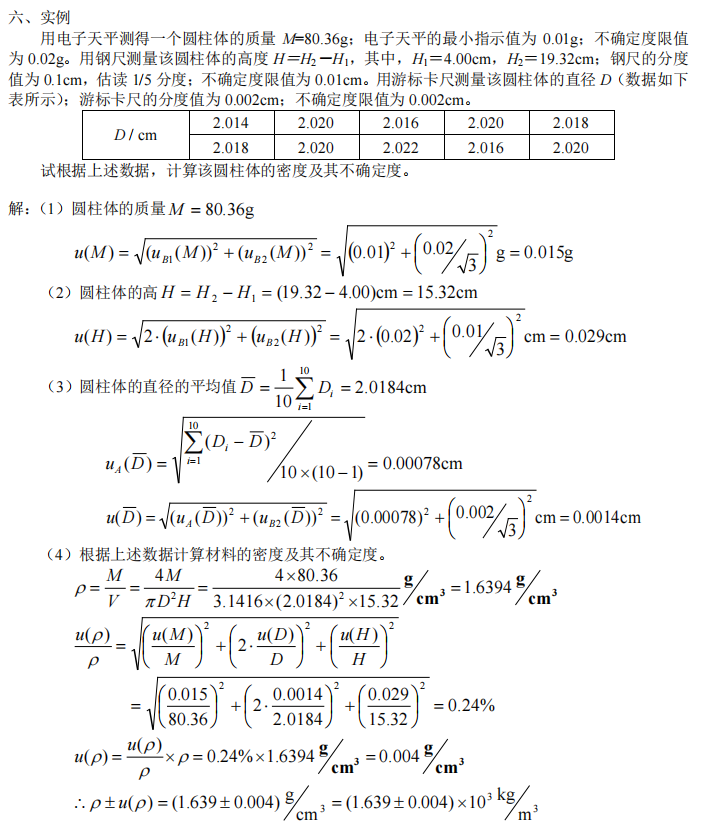
\includegraphics[width=1\linewidth]{C:/Users/Administrator/Desktop/VScode/LaTeX/LatePic/SJCLLT}
		\caption*{}
		\label{fig:sjcllt}
	\end{figure}
	
 \end{document}